\documentclass[12pt]{article}
\usepackage{amsmath,amsfonts,times}
\usepackage{graphicx,color,tikz,pgfplots}
\usepackage[paperwidth=8.1cm,paperheight=8.1cm,lmargin=0in,rmargin=0in,tmargin=0.in,bmargin=0.in]{geometry}
\usepackage{bm}
\usetikzlibrary{arrows,shadings,shapes.arrows,decorations.pathreplacing,calc, positioning}
\usepgfplotslibrary{fillbetween}

\begin{document}
\centering
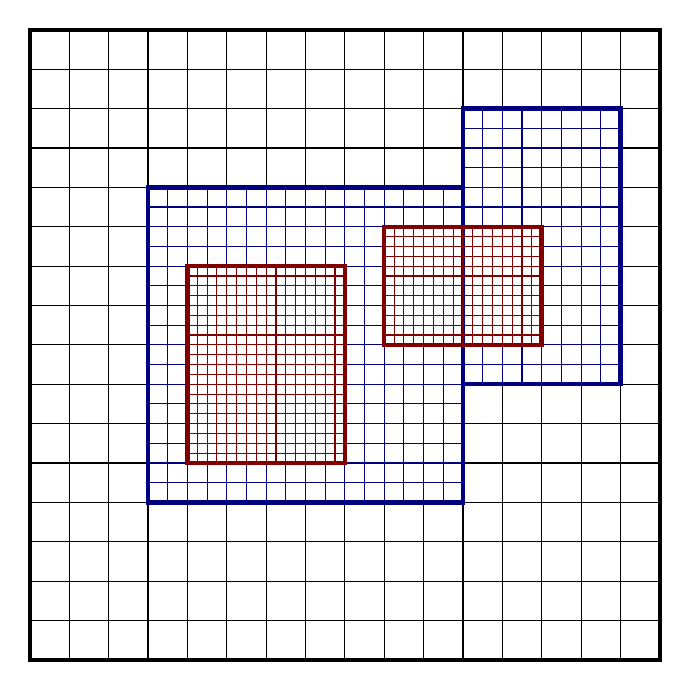
\begin{tikzpicture}[on grid]

  % Parent grid
  \draw[step=5mm, black, thin] (0,0) grid (8,8); %defining grids
  \draw[black,ultra thick] (0,0) rectangle (8,8);%marking borders

  % Nested grid 1, level 1
  \draw[step=2.5mm, blue!50!black, thin] (1.5,2) grid (5.5,6);  %Nested grid 1
  \draw[blue!50!black, ultra thick] (1.5,2) rectangle (5.5,6);%marking borders

  % Nested grid 2, level 1
  \draw[step=2.5mm, blue!50!black, thin] (5.5,3.5) grid (7.5,7);  %Nested grid 1
  \draw[blue!50!black, ultra thick] (5.5,3.5) rectangle (7.5,7);%marking borders

  % Nested grid 1, level 2
  \draw[step=1.25mm, red!50!black, thin] (2.0,2.5) grid (4.0,5);  %Nested grid 1
  \draw[red!50!black, ultra thick] (2.0,2.5) rectangle (4.0,5);%marking borders

  % Nested grid 2, level 2
  \draw[step=1.25mm, red!50!black, thin] (4.5,4.0) grid (6.5,5.5);  %Nested grid 1
  \draw[red!50!black, ultra thick] (4.5,4.0) rectangle (6.5,5.5);%marking borders

  \clip(0,0) rectangle (8,8);
%  \draw[black, ultra thick, draw=black, fill=green!50!black, fill opacity=0.5] (8.0,0.0) circle (4.5cm);
\end{tikzpicture}

\end{document} 
